% ! TeX root = ../thesis-main.tex
%----------------------------------------------------------------------------------------
\chapter{State of the art}
\label{chap:state-of-the-art}
%----------------------------------------------------------------------------------------

In the field of aggregate programming\cite{aggregate-programming}, multiple frameworks, tools, and experiments have been developed and made available as public resources to support a wide variety of use cases, using different languages and design approaches.
%
Some of the prominent examples, that can be considered state of the art, are \textit{ScaFi}\footnote{\url{https://github.com/scafi/scafi}}\cite{scafi}, \textit{Protelis}\footnote{\url{https://github.com/Protelis/Protelis}}\cite{protelis} and, \textit{FCPP}\footnote{\url{https://github.com/fcpp/fcpp}}\cite{fcpp}.
%
In this chapter, each of these tools is briefly described in their fundamental characteristics, with a particular emphasis on ScaFi, which constitutes the direct parent to \this, as discussed in \Cref{chap:background}.

Each of these libraries is backed by a solid, coherent theoretical foundation, that provides theoretical consistency and guarantees the emergence of fundamental properties in derived work.
%
This theoretical foundation that serves as the basis for all cited implementations except Collektive is the \ac{FC}\cite{fc}, in particular its higher-order version, the \ac{HFC}\cite{hofc}.
%
\ac{FC}, as well as its variants, is a type-safe, formal language for aggregate programming\cite{fc, from-dc-to-fc-and-ap} presented with its operational and denotational semantics, respectively describing the local and global interpretation of field expressions\cite{from-dc-to-fc-and-ap}.
%
The key aspect of \ac{FC} is the possibility, from a developer perspective, to focus on the denotational semantics of field constructs, completely abstracting away from the local interpretation of expressions and implementation of the constructs.
%
In recent years, a new formal language has been developed, called \ac{XC}\cite{xc}, which is a promising evolution of \ac{FC} that has the potential to supersede \ac{FC} entirely given that \ac{XC} is a simpler yet more expressive language that can be used to implement all the \ac{FC} constructs while retaining their original semantics.
%
\this, as well as the aforementioned \textit{Collektive}, is based on this newer formal language, as discussed in \Cref{chap:background}, where \ac{FC} and \ac{XC} are briefly compared.
%
Some additional experiments with the implementation of \ac{XC} already exist, such as \textit{imperative-xc}\footnote{\url{https://github.com/cric96/imperative-xc}} and \textit{XC: Scala DSL Implementation}\footnote{\url{https://github.com/scafi/artifact-2021-ecoop-xc}}\cite{xc-experiment-with-scafi}, from which \this takes inspiration for the implementation of the \ac{VM} that executes the aggregate program rounds, as detailed in \Cref{chap:implementation}.

\section{Protelis}
TODO

\section{FCPP}
TODO

\section{ScaFi}

\textit{ScaFi} (\textit{Sca}la \textit{Fi}elds) is an aggregate programming framework featuring an internal \ac{DSL} written in pure Scala 2.
%
Besides the \ac{DSL}, which represents the core of ScaFi, the framework offers additional components for the simulation, visualization, and deployment of aggregate programs.

TODO

\begin{figure}
    \centering
    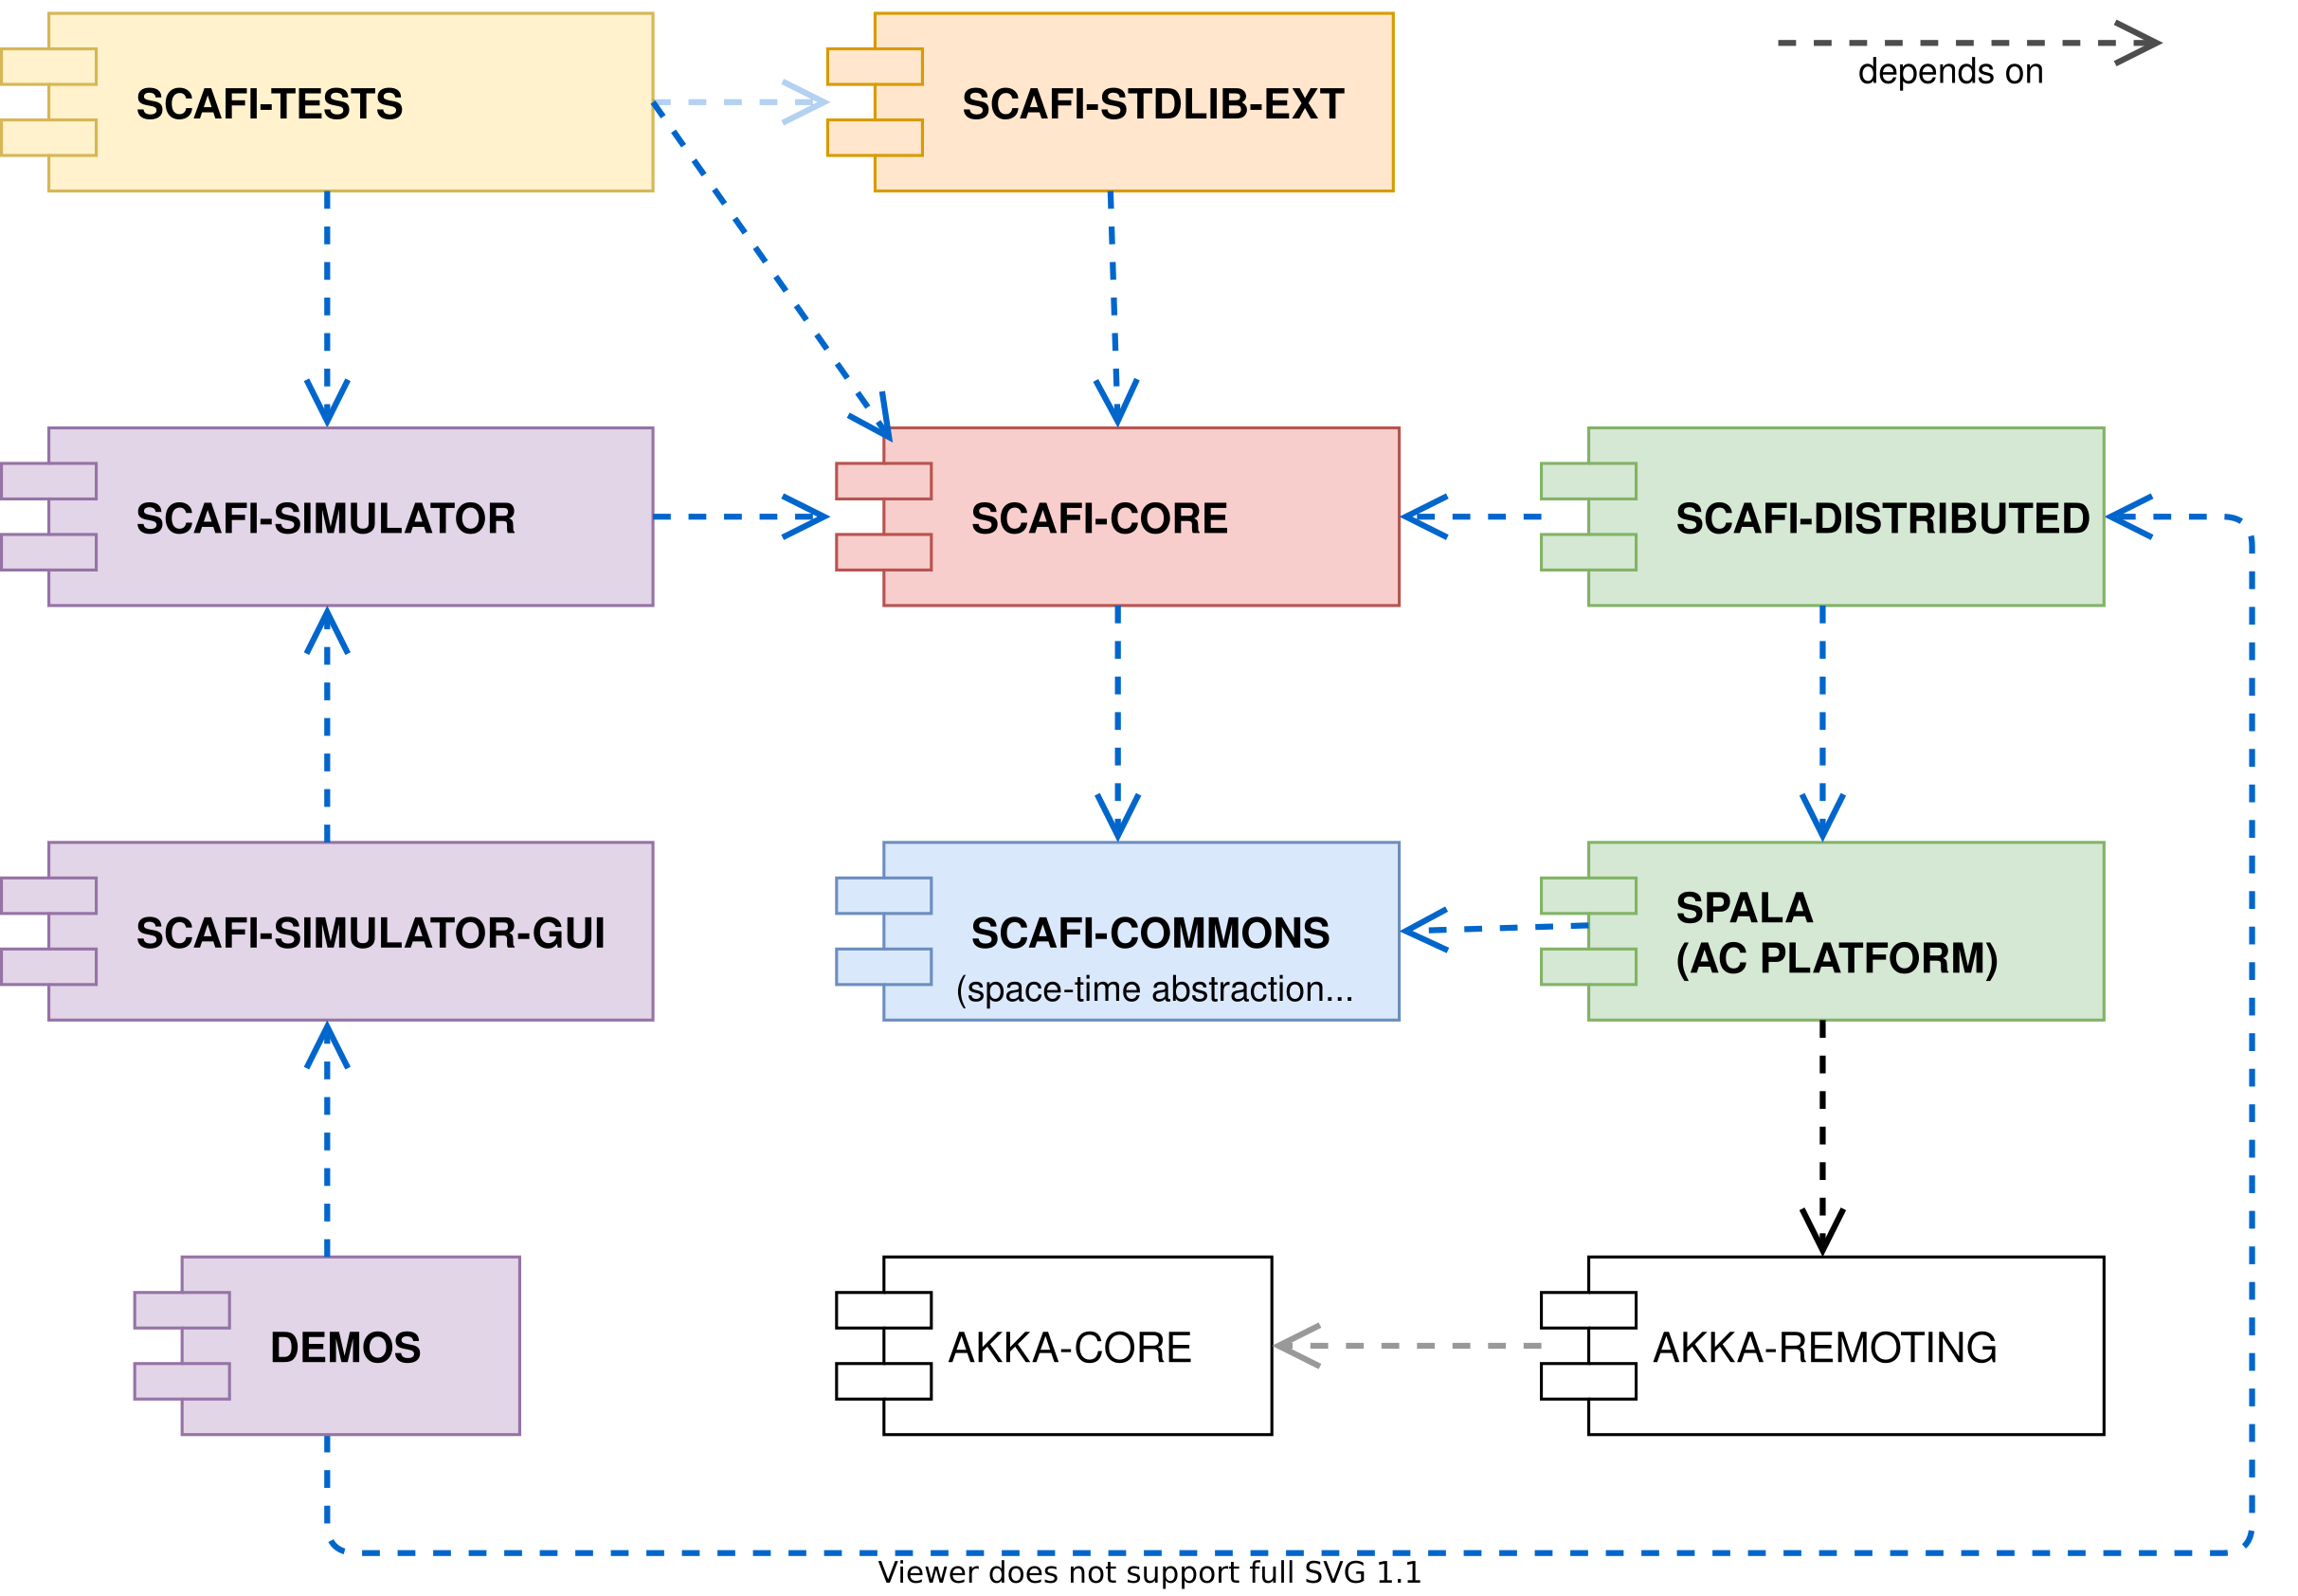
\includegraphics[width=.8\linewidth]{figures/scafi-project-org.drawio.png}
    \caption{Some random image}
    \label{fig:random-image2}
\end{figure}

